% Title:    A LaTeX Template For Responses To a Referees' Reports
% Author:   Petr Zemek <s3rvac@gmail.com>
% Homepage: https://blog.petrzemek.net/2016/07/17/latex-template-for-responses-to-referees-reports/
% License:  CC BY 4.0 (https://creativecommons.org/licenses/by/4.0/)
\documentclass[10pt]{article}
\usepackage{geometry}
\geometry{margin=1in}

% Allow Unicode input (alternatively, you can use XeLaTeX or LuaLaTeX)
\usepackage[utf8]{inputenc}
\usepackage{csquotes}

\usepackage{microtype,xparse,tcolorbox}
\newenvironment{reviewer-comment }{}{}
\tcbuselibrary{skins}
\tcolorboxenvironment{reviewer-comment }{empty,
  left = 1em, top = 1ex, bottom = 1ex,
  borderline west = {2pt} {0pt} {black!20},
}
\ExplSyntaxOn
\NewDocumentEnvironment {response} { +m O{black!20} } {
  \IfValueT {#1} {
    \begin{reviewer-comment~}
      \setlength\parindent{2em}
      \noindent
      \ttfamily #1
    \end{reviewer-comment~}
  }
  \par\noindent\ignorespaces
} { \bigskip\par }

\NewDocumentCommand \Reviewer { m } {
  \section*{Comments~by~Reviewer~#1}
}
\ExplSyntaxOff
% \AtBeginDocument{\maketitle\thispagestyle{empty}\noindent}

% You can get probably get rid of these definitions:
\newcommand\meta[1]{$\langle\hbox{#1}\rangle$}
\newcommand\PaperTitle[1]{``\textit{#1}''}


\begin{document}


\noindent \textbf{Pacific Symposium on Biocomputing 2018}

\noindent October 2, 2017 \\

\noindent Dear Organizers,\\

We are pleased to resubmit our manuscript entitled, \PaperTitle{An Ultra-Fast and Scalable Quantification Pipeline for Transposable Elements from Next Generation Sequencing Data,} for the publication in the proceedings of \textbf{Pacific Symposium on Biocomputing 2018.}
We also thank the reviewers for their careful reading and constructive comments.  Please find our point-to-point response below.  \\

\noindent Zhandong Liu, Ph.D. \\
Assistant Professor\\
Baylor College of Medicine \\
Jan and Dan Duncan Neurological Research Institute \\
1250 Moursund St., Houston, Texas, 77030 

\begin{figure}[h]
    
\includegraphics[width=0.2\textwidth]{zdsig.png}
\end{figure}

\Reviewer{\#1}
\begin{response}{Appropriateness for PSB: This article proposed a new bioinformatics pipeline for the quantification of transposable elements from NGS data. The article addresses the challenges of quantifying TE patterns in large-scale sequencing data, therefore fits the scope of PSB and the session very well.}
We appreciate the reviewer's reading and positive assessment of our manuscript.
We thank the reviewer for the time spent and positive feedback.
\end{response}
\begin{response}{Presentation: This article is very well written. It flows well and pleasant to read. The figures, tables, and equations are nicely presented and helpful. The scope of the approach is clearly stated but the limitations are not discussed specifically. The article compared their SalmonTE pipeline to TEtranscripts and showed that the quantification performance is comparable but at a much less computational cost. 
It would be helpful to extend the discussion on the methodological differences between those two approaches and explain the improved computational efficiency.}
To address the reviewer's concern, we have added a paragraph which describes differences between SalmonTE and TEtranscripts in the method section.
\\

\textbf{[In the revised manuscript]} 
\textbf{(In the last paragraph of page 2)} 

\textcolor{red}{
The proposed pipeline consists of three parts: library preparation, quantification, and statistical analysis (Figure 1). To increase the usability and to enable parallel processing for multiple RNA-seq reads files, we adopted the Snakemake workflow system and wrote a script based on the execution rule of Snakemake for the TE quantification.$^{21}$ In contrast to TEtranscripts, SalmonTE starts with raw RNA-seq files, and does not need any additional pre-processing for a given sequence file. Moreover, TEtranscripts requires a modified GTF files based on RepeatMasker database.$^{22}$ SalmonTE only needs the FASTA file of cDNA (complementary DNA) sequences of each TE. The entire source code and executable scripts are available at https://github.com/hyunhwaj/SalmonTE.}

\end{response}
\begin{response}{Significance: Through the comparisons with the most widely used approach, it was shown that the new proposed pipeline can achieve comparable accuracy. The proposed approach also has the potential to scale up for larger NGS datasets.}
We appreciate the reviewer's reading and positive assessment of our manuscript.
\end{response}
\begin{response}{Originality: The core algorithm Salmon was proposed previously by another research group so the originality of this article is limited. However it proposed a new bioinformatics pipeline that was shown to accelerate TE quantification. It will be a nice addition to the research community.}
 
We agree with the reviewer's opinion that the originality of the paper is limited as a methodological paper. We also agree that the main contribution of our study is to develop a practical bioinformatics pipeline for the research community. 
\end{response}

\begin{response}{Additional Comments for the Authors: The manuscript is well written and the approach is well designed and effective. It will be welcomed by the PSB audience.}
We appreciate the reviewer for the positive assessment. 
\end{response}

\Reviewer{\#2}
\begin{response}{Appropriateness for PSB: This is an interesting paper, but I’m not sure if this is relevant to the "Challenges of Pattern Recognition in Biomedical Data" session.}
We partially agree with the reviewer's concern for the relevance of the section, but we believe that our manuscript is appropriate to submit this section due to following reasons:

\begin{enumerate}
\item Transposon element can be considered as a pattern on the genome, and the quantification of the pattern from RNA-seq is very challenging because it is repetitive and causes a computational problem.
\item We also discussed the application of our pipeline to a large-scale dataset
in agreement with one of the session interests 
``Challenges of computational resource requirements for large-scale and high-dimensionality data analysis.''
\end{enumerate}
\end{response}
\begin{response}{Presentation: In general, there are appropriate tables and figures. However, authors need to provide more detailed description in the legend for each figure. Additionally, it needs more proof-readings since there are a few typos and grammar mistakes.}
We have carefully revised the entire manuscript to provide more detail on each figure.
\end{response}

\begin{response}{Significance: Identifying/quantifying transposable elements is an important task. Biologically, transposable elements play important roles in several diseases. In addition, there was a great improvement in the context of computationally advance.}
We appreciate the reviewer for the positive assessment. 
\end{response}

\begin{response}{Originality: My enthusiasm about this paper was a bit diminished due to the lack of novelty. I think making a new pipeline that used existing tools or methods and comparing it to only one previous method (TEtranscripts) is incremental. Authors should compare the proposed pipeline to other methods.}

Based on the reviewer's comment, we have performed additional experiments with other methods.  
\\

\textbf{[In the revised manuscript]} 

\textbf{(In the first paragraph of ``3.3. SalmonTE~guarantees a reliable TE expression estimation'')}

\textcolor{red}{
For the quantification accuracy comparison, we first took estimated abundance of 8 TEs from each quantification tool. Those 8 TEs have measured by Reverse Transcription-quantitative Polymerase Chain Reaction (RT-qPCR) for the relative expression validation in [6]. We ob- served SalmonTE performs better than other tools ($r^2 = 0.9796$, Figure 2 and Table 1), but it is slightly better than TEtranscripts. However, we can found that SalmonTE outperforms that case of TEs which are weakly down-regulated (DM1731\_I and HETA) and TEtranscripts does not provide a correct estimation in this case.}
\\

\textbf{(Figure 2 in page 6)}
\begin{figure}[h]
\centerline{
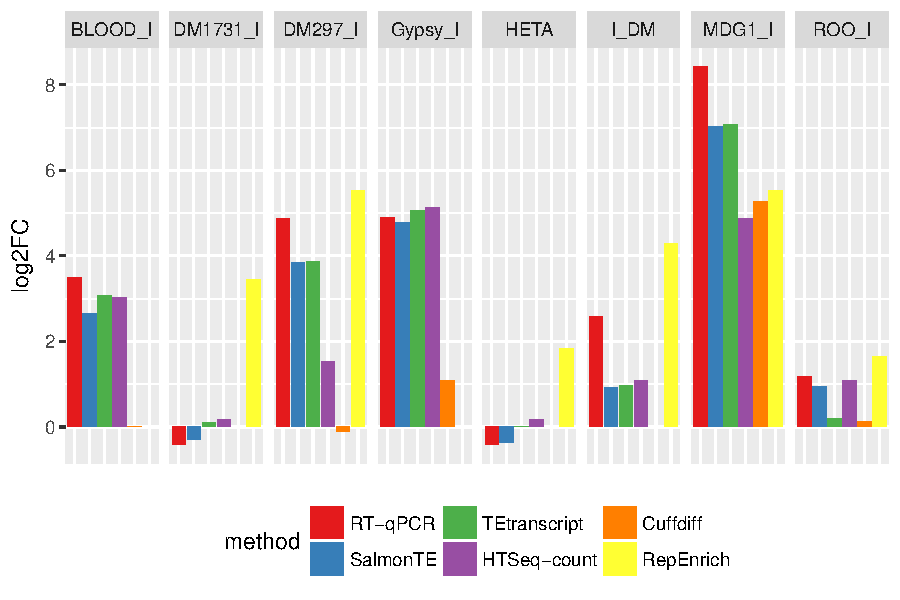
\includegraphics[width=10cm]{fig_bar}
}
\end{figure}


\textbf{(Table 1 in page 7)}
\begin{table}[h]
\begin{center}
\begin{tabular}{l|lllll}
	\hline
	Method    & SalmonTE & TEtranscripts & HTSeq-count & Cuffdiff & RepEnrich  \\ \hline
	 $r^2$ & 0.9796 & 0.9658 & 0.8514 & NA & NA \\ \hline
\end{tabular}
\end{center}
\end{table}


\end{response}

\begin{response}{Additional Comments for the Authors: This is an interesting paper and will be very helpful to the community as long as they provide more comparison results.}
We appreciate the reviewer's reading and positive assessment of our manuscript.
\end{response}
% Thank you

\Reviewer{\#3}

\begin{response}{Appropriateness for PSB: While it is clear the authors made a significant advance in the area of quantifying TEs from RNA-seq data, it was not clear that this leads to any new biological conclusions.}
The focus of this manuscript is to develop a new bioinformatics tool to identify and quantify transposable elements from 
transcriptome data.  We appreciate the reviewer's comment that our tool is a significant advance in this area.  The discovery of new biology is out of the scope for this work. But we do have another manuscript under-review where we applied our method to systematically identify new TE patterns in Alzheimer's Disease.
\end{response}


\begin{response}{Presentation: There were spelling and grammar errors in a number of places.

Second sentence of abstract. 
}

We are sorry for the typos in the paper.  We have corrected all the grammar errors to our best. 
\end{response}

\begin{response}{
I thought the methods were poorly described for parts 2.1 and 2.2. It was very difficult to make sense of what was being described. The results need to be described better. My advice would be to describe your reasoning as to why the analysis was done, how it was performed, the result and what is says about the method and biology. This was not always stated, but should have been or made more clear.}

We have completely revised \textbf{2.1.} and  \textbf{2.2.} to help better understanding of mathematical details about the quantification algorithm.\\


\textbf{[In the revised manuscript]} 

\textbf{(The paragraph of ``2.1. Transposable Element Library Preparation'' in page 3)}

\textcolor{red}{
As we mentioned earlier, SalmonTE needs a library of TE which consists of FASTA file of cDNA sequences to create an index for the TE quantification. SalmonTE provides Salmon index files of TE libraries of Homo sapiens and Drosophila melanogaster. We introduce how we generate the index files in this subsection. First, we collected FASTA files of the TE cDNA sequences for Homo sapiens and Drosophila melanogaster from Repbase (version 22.06).$^{22}$ We hypothesized that it is hard to estimate several TEs which replicate without an RNA intermediate from RNA-seq sample, so we have excluded those kinds of elements: simple repeats and multi-copy genes, and DNA transposable. After collecting the cDNA sequences, we manually curated clades of each TE based on the repeat class annotation of Repbase.
As a result, the generated TE library index files contains 687 TEs for Homo sapiens and 163 TEs for Drosophila melanogaster.}

\end{response}

\begin{response}{Significance: While it is important to understand how TEs are connected to disease, it is unclear how the methodology was able to illustrate that. I think the authors could have illustrated the biological significance by comparing their tool to another tool and illustrate they reduced the false discovery rate of detecting TEs. Why not perform a new analysis that was previously unattainable to understand when quantification took a long time? Interestingly, the main motivation for speeding things up was so it could scale but I don’t really see them illustrate using their method in a big meta-analysis. }

The main focus of our manuscript is to develop a tool that is fast and accurate.  Meta-analysis on large dataset is out of the scope.  We do have another manuscript under-review where a meta-analysis on AD transcriptome is carried out and new biology was discovered and validated using model organisms.  

The lack of meta-studies in the area of TE analysis is primary due to the challenge of slow running time.  Armed with this new tool, we expect to see many labs running their own meta analysis without the need of super computers. 
\end{response}

\begin{response}{Originality: The authors do compare their method to a similar method and find it was faster but didn’t quantify TEs any better.}
% Showing example Salmon and Kalisto, add a sentence 
The key challenge here is the speed.  The state of the art approach runs slow and it will take a couple of hours for a single sample of a standard RNA-seq dataset. 
Like many great bioinformatics tools, our main contribution is the speed.  With this faster tool, we can now analyze many large datasets. 

To address the reviewer's concern on accuracy, we also included a new figure and a table in which we compared SalmonTE to other methods.  This new result demonstrates that SalmonTE outperformed all other methods in TE quantification accuracy. 
\end{response}

\begin{response}{Additional Comments for the Authors: The approach seemed to be implemented well but the methods section was very difficult to understand.}
We have carefully revised the method section. We also changed the titles of each result section to reflect the findings from our experiments. 

\textcolor{red}{
\begin{itemize}
	\item The title of 3.2. became ``Computational experiment setup''.
    \item The title of 3.3. became ``SalmonTE guarantees a reliable TE expression estimation''.
    \item The title of 3.4. became ``SalmonTE shows a better scalability in the speed benchmark dataset''.
	\item The title of 3.5. became ``Discover differentially expressed TEs in ALS cell line''.
\end{itemize}}
\end{response}

\begin{response}{
Minor comments: Abstract, neurodegenerative is spelled wrong. Although most of TE studies contain a few RNA-seq... should be Although most of TE studies only contain a few RNA-seq... 

I would recommend re-arranging the introduction to discuss the meta-analysis then get into the details of scaling. It would be better to describe what is motivating you to do the study then get into the scaling. }
We fixed the typo of `neurodegenerative' and correct the sentence starts with `Although most of TE studies\dots'

We also added the rationale for meta-analysis in the introduction. 
% Have to arrange the introduction
\end{response}

\end{document}